\section{Final separation is often written late}

Once the final answer has become a persistent contender, the trajectory is not finished. The final-pair gap can still be small, and later layers often add much of the eventual separation. We measure this by summing positive increases in the final winner-versus-runner-up gap and asking how much of that positive write occurs after key events.

\begin{figure}[tbp]
\centering
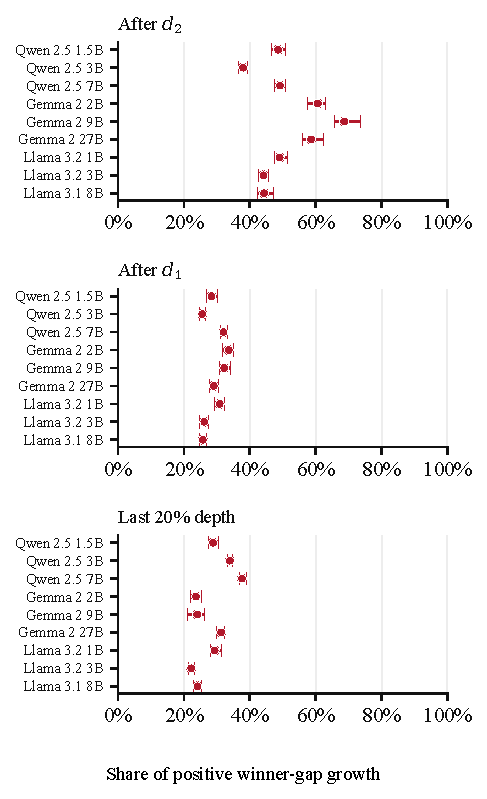
\includegraphics[width=\linewidth]{figure3_late_write.pdf}
\caption{\textbf{Much of the final winner-gap growth occurs after contender status.} Each point is a model median; intervals are 95\% bootstrap intervals. The broad panel shows that contender formation does not imply immediate isolation.}
\label{fig:late-write}
\end{figure}

The pooled median share of positive winner-gap growth written after $d_2$ is \PooledWriteAfterDTwo{}. Even after persistent top-1 status, the median remaining positive write is \PooledWriteAfterDOne{}. This makes late write a natural companion to the persistence-depth result: the model can have selected the eventual answer while still continuing to strengthen it.

This is why late write is not redundant with persistent winner status. Persistent top-1 says that the final answer has stopped losing to another option; late write says that the gap separating it from the runner-up is still being actively increased.

This is a readout-space statement. It does not by itself identify which internal components create the late write. The instrumented panel below asks that narrower mechanistic accounting question.
